\documentclass[english]{article}
\usepackage{geometry}
\usepackage{inputenc}
\usepackage{csquotes}
\usepackage{hyperref}
\geometry{verbose,tmargin=3.5cm,bmargin=4cm,lmargin=3.8cm,rmargin=3.8cm}
\newcommand\graphwidth{0.49\textwidth}
\usepackage[backend=biber,style=ieee]{biblatex}
\addbibresource{sources.bib}
\makeatletter
\usepackage{url}
\usepackage{graphicx}
\usepackage{caption}
\usepackage{wrapfig}
\usepackage{subcaption}
\makeatother
\usepackage{babel}
\usepackage{amsmath}
\usepackage{amsthm}
\newtheorem{theorem}{Theorem}[section]
\newtheorem{lemma}[theorem]{Lemma}
\newtheorem{conjecture}{Conjecture}
\newtheorem{property}{Property}
\newtheorem{corollary}{Corollary}[property] % Use theorem counter as `parent`
\usepackage{algorithm}
\newcommand{\Desc}[2]{\State \makebox[2em][l]{#1}#2}
\usepackage[noend]{algpseudocode}
\makeatletter
\def\BState{\State\hskip-\ALG@thistlm}
\makeatother


\begin{document}
	
	\title{Multi-Agent Pathfinding with Matching using Increasing Cost Tree Search}
	\author{
		Thom van der Woude$^1$\\[2ex]
		\normalsize{Supervisors: Jesse Mulderij$^1$ Mathijs de Weerdt$^1$}
	}
	\date{
		\normalsize{$^1$TU Delft\\
		t.b.vanderwoude@student.tudelft.nl\\\{j.mulderij, m.m.deweerdt\}@tudelft.nl\\[2ex]
		}
	}
	
	\maketitle
	
	\begin{abstract}
		\noindent Both the assignment problem and the multi-agent pathfinding problem are common problems in the fields of robotics and transportation. The joint problem of multi-agent pathfinding extended with the assignment of goals to agents, matching, is something that has not been studied much; few methods exist today that solve it. In this work, two types of algorithms based on the Increasing Cost Tree Search (ICTS) algorithm for multi-agent pathfinding are presented that can optimally solve this joint problem: exhaustive algorithms that reduce the problem to solving many multi-agent pathfinding problems using regular ICTS, and algorithms that search a generalized increasing cost tree. These are compared to each other experimentally on a set of grid maps, and it is shown that exhaustive methods typically outperform the generalized ICTS. Lastly, an exhaustive ICTS algorithm is compared to alternative algorithms based on other multi-agent pathfinding approaches to put its performance into the broader context of algorithms for multi-agent pathfinding with matching.
	\end{abstract}
	
	\section{Introduction}
	Finding a shortest path between two vertices on a graph is a fundamental problem that appears in many contexts like GPS navigation \cite{sturtevant2010} and network routing \cite{broch1998}. In some applications like autonomous aircraft towing \cite{morris2016} and train unit routing in shunting yards \cite{mulderij2020}, planning agents separately can result in conflicts between agents as they follow their paths. To prevent such conflicts, agents have to be planned together to find a combination of non-conflicting paths. The problem of finding such a combination is the Multi-Agent Pathfinding (MAPF) problem \cite{stern2019}. In finding optimal solutions, one of two objectives is typically optimized: the makespan which is the cost of the longest path, or the Sum of Individual path Costs (SIC). Algorithms for optimally solving MAPF include Increasing Cost Tree Search \cite{sharon2013}, Conflict-Based Search \cite{sharon2015} and Branch-and-Cut-and-Price \cite{lam2019}.
	
	As observed by \cite{ma2016b}, in real-world applications of MAPF such as warehouse robotics \cite{wurman2007} goals are often assigned to teams of agents instead of single agents as in standard MAPF. Using MAPF in such applications requires pre-assignment of goals to agents using the Hungarian Algorithm \cite{kuhn55} or similar methods, but such approaches are suboptimal as the true cost of a given matching can only be found by solving the corresponding MAPF instance. 
	\begin{wrapfigure}[21]{r}{.25\textwidth}
		\vspace{-10pt}
		\begin{minipage}{\linewidth}
			\centering\captionsetup[subfigure]{justification=centering}
			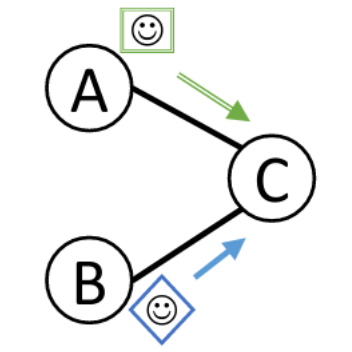
\includegraphics[width=\linewidth]{img/vertex-conflict}
			\subcaption{Vertex conflict}
			\label{fig:conflictsa}\par\vfill
			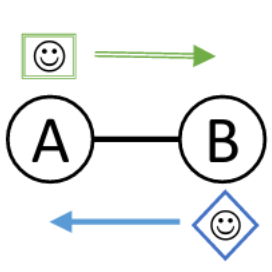
\includegraphics[width=0.75\linewidth]{img/edge-conflict}
			\subcaption{Edge conflict}
			\label{fig:conflictsb}
		\end{minipage}
		\vspace{-10pt}
		\caption{Two types of conflicts between agents from \cite{stern2019}.}\label{fig:conflicts}
	\end{wrapfigure}
	Ma and Koenig \cite{ma2016} formulate the joint problem of finding the optimal makespan solution across all possible matchings as the combined target-assignment and pathfinding (TAPF) problem. They also present the Conflict-Based Min-Cost-Flow (CBM) algorithm for solving TAPF. 
	In CBM, the Meta-Agent variant of CBS \cite{sharon2015} is used as a high-level search framework; in the low-level search, single teams are planned in polynomial time as constrained anonymous MAPF instances using a max-flow approach \cite{yu2013}. The experimental results reported in \cite{ma2016} indicate that CBM scales well as the number of agents and the sizes of teams increase; although in addition to grid instances with 10\% of tiles being blocked, Kiva \cite{wurman2007} instances are also solved, it remains to be seen how CBM performs in scenarios with more obstacles and more maze-like scenarios such as the Moving AI maps \cite{sturtevant2012}.
	
	Nonetheless, CBS successfully being used to solve TAPF raises two questions: Can MAPF algorithms other than CBS be used to solve TAPF? Can CBS or other MAPF algorithms be used to solve TAPF minimizing the SIC instead of the makespan? For this latter problem that will be referred to as Multi-agent Pathfinding with Matching (MAPFM), no methods are described in the literature. 
	
	This work presents two types of algorithms based on ICTS \cite{sharon2013} that optimally solve MAPFM, and is part of a study in which other algorithms in addition to ICTS were taken as starting points for MAPFM algorithms. Those of the first type exhaustively enumerate matchings and use a variant of ICTS as a subroutine; those of the second type are based on an extension of ICTS itself to support matching, ICTS-m. The properties of both classes of algorithms as well as ICTS more generally are discussed, followed by an experiment in which a selection of algorithm variants is compared. Additionally, one exhaustive ICTS algorithm is compared to MAPFM algorithms based on CBM \cite{ma2016}, M* \cite{wagner2011}, A*+OD+ID \cite{standley2010} and EPEA* \cite{goldenberg2014}. 
	
	
	
	
	
	%To date, methods solving TAPF and similar problems \cite{henkel2019} use CBS. 
	
	%Can other MAPF algorithms be used to solve TAPF?
	
	%The successful application of CBS to solving TAPF begs the question: \textit{can other MAPF algorithms such as Increasing Cost Tree Search (ICTS) \cite{sharon2013} serve as the basis for a TAPF algorithm?}
	
	% remains the question of how multi-agent pathfinding with matching (MAPFM) minimizing the SIC
	
	
	
	%To date, no method is described in the literature for solving a related problem: multi-agent pathfinding with matching minimizing SIC.
	
	%the multi-agent pathfinding with matching problem minimizing SIC
	
	%Multi-agent pathfinding with matching (MAPFM) minimizing SIC. 
	%describe a related problem in a factory setting where agents have to first move from their start location to the start position of a task.
	
	%In this work, a problem related to TAPF will be discussed, namely multi-agent pathfinding with matching minimizing SIC (MAPFM). This is related to the problem described by 
	
	%To date, the Task Conflict-Based Search algorithm \cite{henkel2019} based on CBS is the on
	
	%, as well as optimal ICTS-based a 
	
	%For an analogous problem, multi-agent pathfinding with matching using the SIC objective (hereafter MAPFM)
	
	
	%Henkel et al. \cite{henkel2019} describe the Task Conflict-Based Search algorithm for the 
	
	
	
	
	%This work is the outcome of a search for algorithms that optimally solve MAPFM based on ICTS \footnote{To the knowledge of the author, to date, no such algorithm is described in the literature}, which is part of a study in which other algorithms addition to ICTS were taken as starting points for MAPFM algorithms. Two classes of ICTS-based algorithms were found: one based on exhaustive enumeration of matchings using a variant of ICTS as a subroutine, the other based on modifications to the Increasing Cost Tree (ICT) structure and its search. One exhaustive ICTS algorithm is compared to algorithms based on CBM \cite{ma2016}, M*\cite{wagner2011}, A*+OD+ID\cite{standley2010} and EPEA*\cite{goldenberg2014} to put ICTS methods for MAPFM into a broader context.

	\section{Multi-agent Pathfinding with Matching} % Problem description
	\label{mapfm}

	
	A MAPF instance can be defined as follows. Let $G = (V,E)$ be an undirected graph, with each $v\in V$ representing an obstacle-free tile on a 4-connected grid and each $e = (u,v)\in E$ representing a legal move between two such tiles. Let there be $k$ agents $a_1,\ldots,a_k$ with starting locations $s_1,\ldots,s_k$ and goals $g_1,\ldots,g_k$. For each agent $a_i$, a path $\pi_i$ from $s_i$ to $g_i$ is to be found such that all agents' paths $\pi_i$ taken together are non-conflicting and therefore are a solution. In this work, non-conflicting means, in the conflict-terminology of \cite{stern2019}, that there are no vertex conflicts and no edge conflicts, as shown in Figure \ref{fig:conflicts}. Letting $\pi_i^t$ denote the $t$'th node of path $\pi_i$, this means that for $i\neq j$, for all $t$, $\pi_i^t\neq \pi_j^t$ and $(\pi_i^t \neq \pi_j^{t + 1})\lor(\pi_i^{t+1} \neq \pi_j^t)$. To achieve this, each agent $a_i$ may wait during any time step $t$ so that $\pi_i^t = \pi_i^{t+1}$ instead of moving to a grid neighbor. Given a solution $(\pi_1,\ldots,\pi_k)$, a vector of per-agent costs $(c_1,\ldots,c_k)$ can be found. For $\pi_i$, $c_i$ is defined as the time at which $a_i$ reaches $g_i$ for the last time, meaning that for $t \geq c_i$, $\pi_i^{t} = g_i$. 
	For each $c_i$, $c_i \geq c^*_i$ where $c^*_i$ is defined as the cost of a shortest path from $s_i$ to $g_i$.
	
		 \begin{wrapfigure}[9]{r}{.35\textwidth}
		\vspace{-10pt}
		\centering
		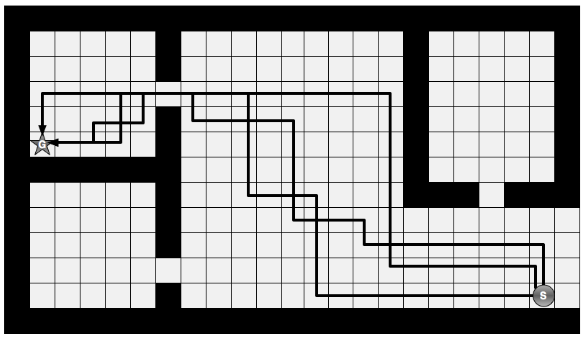
\includegraphics[width=\linewidth]{img/symmetries}
		\caption{Symmetric paths on a 4-connected grid \cite{harabor2010}.}
		\label{fig:symmetries}
	\end{wrapfigure} 
	\subsection{Objectives for MAPF}

	Using the established terminology, the two common objectives for MAPF can be restated as follows:

	\begin{itemize}
		\item Makespan: $\max_{i} c_i$
		\item Sum of individual costs (SIC): $\sum_i c_i$
	\end{itemize}
	In this work, an optimal solution is defined as having minimal SIC.
	

	The mapping from $(\pi_1,\ldots,\pi_k)$ to a SIC is surjective: many cost vectors $(c'_1,\ldots,c'_k)$ might add up to the same SIC as $(c_1,\ldots,c_k)$ and for a given agent $a_i$, there might be many equivalent paths $\pi'_i$ to the goal with cost $c_i$. On uniform-cost 4-grids in particular, there are often many equivalent and symmetrical paths \cite{harabor2010} (see Figure \ref{fig:symmetries}), which is why in single-agent pathfinding, symmetry-breaking methods such as Jump Point Search \cite{harabor2011} are used to speed up the search. In multi-agent pathfinding, having multiple paths per agent of the same cost can, in contrast, be a boon: it means that there are potentially more non-conflicting ways to combine paths of different agents.
	
	\subsection{Extending MAPF with matching}
	With the multi-agent pathfinding problem defined, the MAPFM problem that is the subject of this work can be described as an extension of MAPF.
	
	Let there be $K$ teams $t_1,\ldots, t_K$, where $t_i$ consists of $k_i$ agents with start positions $s_1^i,\ldots,s_{k_i}^i$ together with an equal number of team goals $g_1^i,\ldots,g_{k_i}^i$. Within each team $t_i$, agents $a_j^i$ are to be \textit{matched} to a unique goal $g_k^i$, so that exactly one agent is assigned to each goal within team $i$; once all agents are matched with goals, for each agent $a_j^i$ matched with $g_k^i$, a path from $s_j^i$ to $g_k^i$ is to be found such that all agents' paths taken together are non-conflicting and therefore make up a solution, similarly defined as for MAPF.
	
	MAPFM, being TAPF with a SIC objective, generalizes both MAPF and anonymous MAPF \cite{ma2016}, which is MAPF allowing an agent to move to any goal, a problem that can be solved in polynomial time.
	
	\section{Solving MAPF with Matching using ICTS} % Your contribution
	\label{section:icts-matching}
	In this section, taking ICTS for MAPF as a starting point, two methods to use ICTS to solve MAPFM are described. The first method relies on a reduction from MAPFM to repeated MAPF: an optimal solution to MAPFM corresponds to a matching of agents to goals, so by exhaustively enumerating all matchings and solving these as MAPF instances, an optimal solution to the MAPFM instance can be found. In the second method, the ICT search itself is modified to allow an agent $a_j^i$ to be matched to any $g_k^i$.
	\subsection{Increasing Cost Tree Search}
	\label{icts}
	In Increasing Cost Tree Search \cite{sharon2013}, the two-step mapping from path combination to SIC described in Section \ref{mapfm} is reversed to search for a solution with minimal SIC. This is done by searching for cost vectors corresponding to increasing SIC at the top level and searching for non-conflicting path combinations (solutions) for each cost vector at the bottom level. 
	
	\subsubsection{Top-level search}
	In the top-level search, all possible cost vectors for a given SIC are evaluated by searching an Increasing Cost Tree as depicted in Figure \ref{fig:ict}, starting from $C^* = \sum_i c^*_i$ corresponding to a single root cost vector $(c^*_1,c^*_2,\ldots,c^*_k)$. This root has $k$ children $(c^*_1 + 1,c^*_2,\ldots,c^*_k),(c^*_1,c^*_2 + 1,\ldots,c^*_k),\ldots,(c^*_1,c^*_2,\ldots,c^*_k + 1)$ all of cost $C = C^* + 1$. Searching this ICT breadth-first corresponds to evaluating all possible cost vectors corresponding to increasing cost $C$ starting with $C^*$, guaranteeing optimality of a found solution. When searching up to  cost $C^* + \Delta$, $\mathcal{O}(k^\Delta)$ cost vectors are evaluated. Node evaluation corresponds to performing a low-level search for a solution $(\pi_1,\ldots,\pi_k)$ corresponding to the node cost vector $(c_1,\ldots,c_k)$.
	
	\begin{figure}[t]
		\centering
		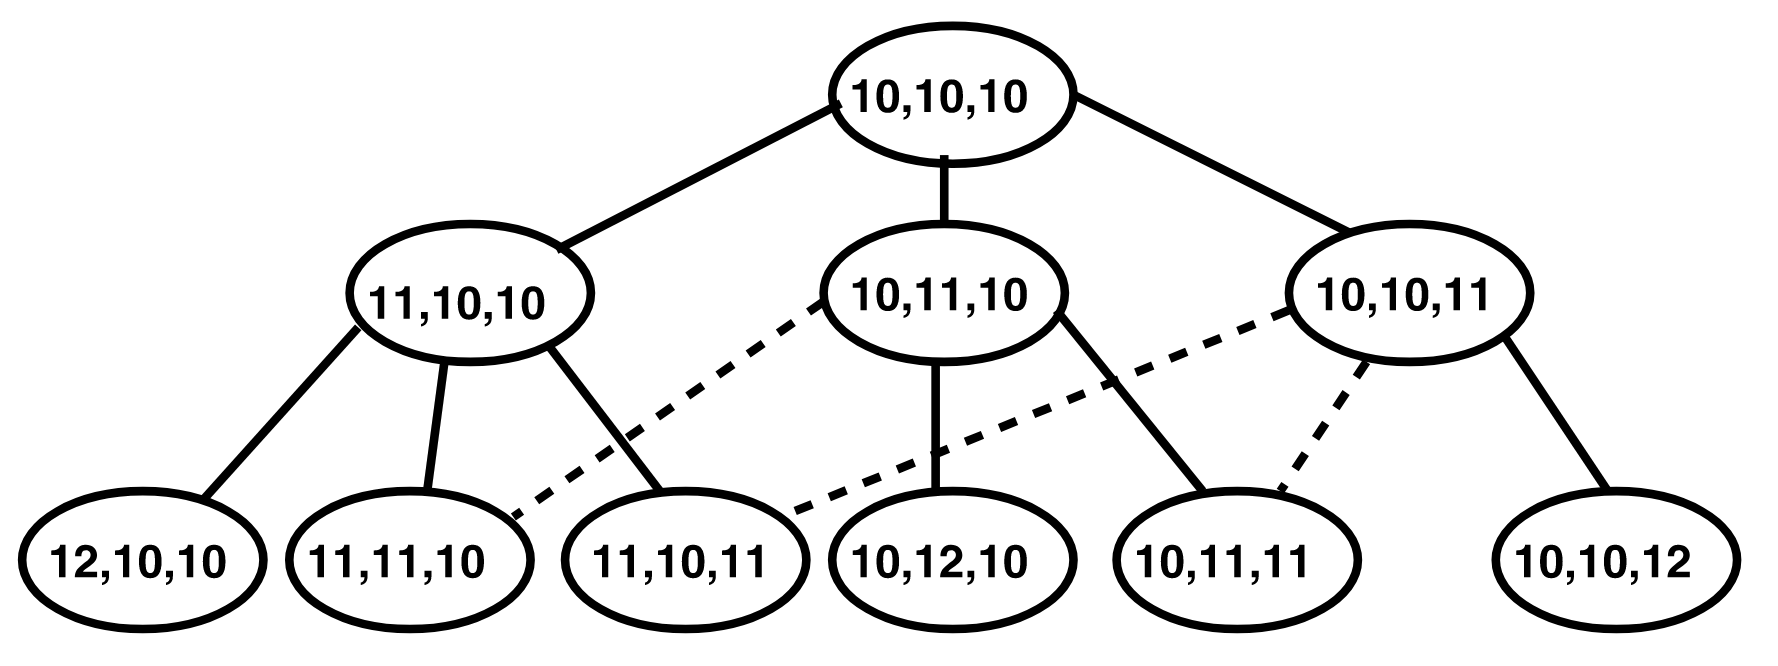
\includegraphics[width=0.5\linewidth]{img/ict}
		\caption{Increasing Cost Tree for three agents \cite{sharon2013}.}
		\label{fig:ict}
		\vspace{-30pt}
	\end{figure}
	\begin{figure}
		
	\end{figure}
	
	
	\begin{figure}[b]
		\centering
		\begin{subfigure}{0.2\textwidth}
			\centering
			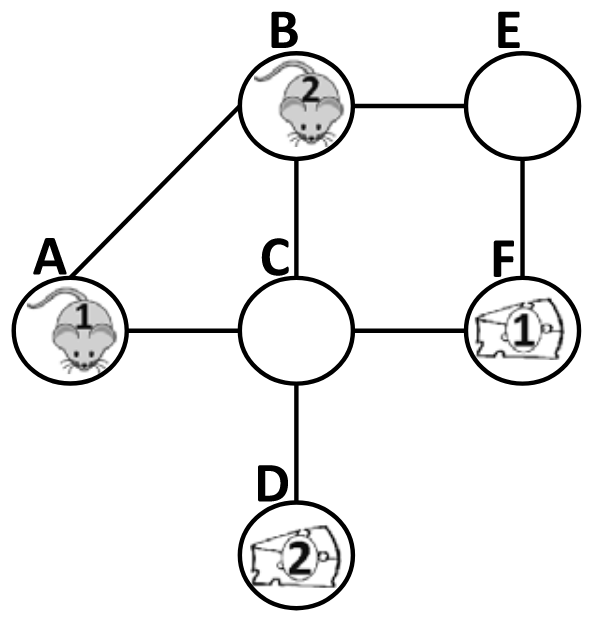
\includegraphics[width=\linewidth]{img/mdds1}
			\caption{An example problem.}
			\label{fig:problem}
		\end{subfigure}
		\hfill
		\begin{subfigure}{0.3\textwidth}
			\centering
			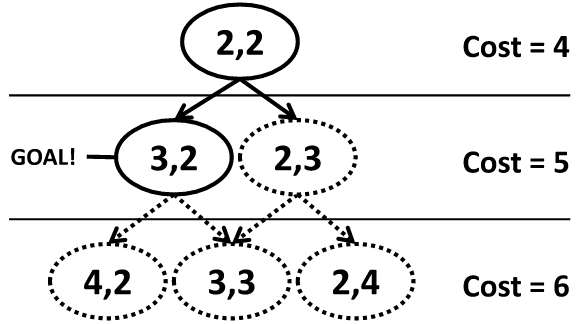
\includegraphics[width=\linewidth]{img/ict2}
			\caption{The corresponding ICT with solution node $(3,2)$.}
			\label{fig:ict2}
		\end{subfigure}
		\hfill
		\begin{subfigure}{0.4\textwidth}
			\centering
			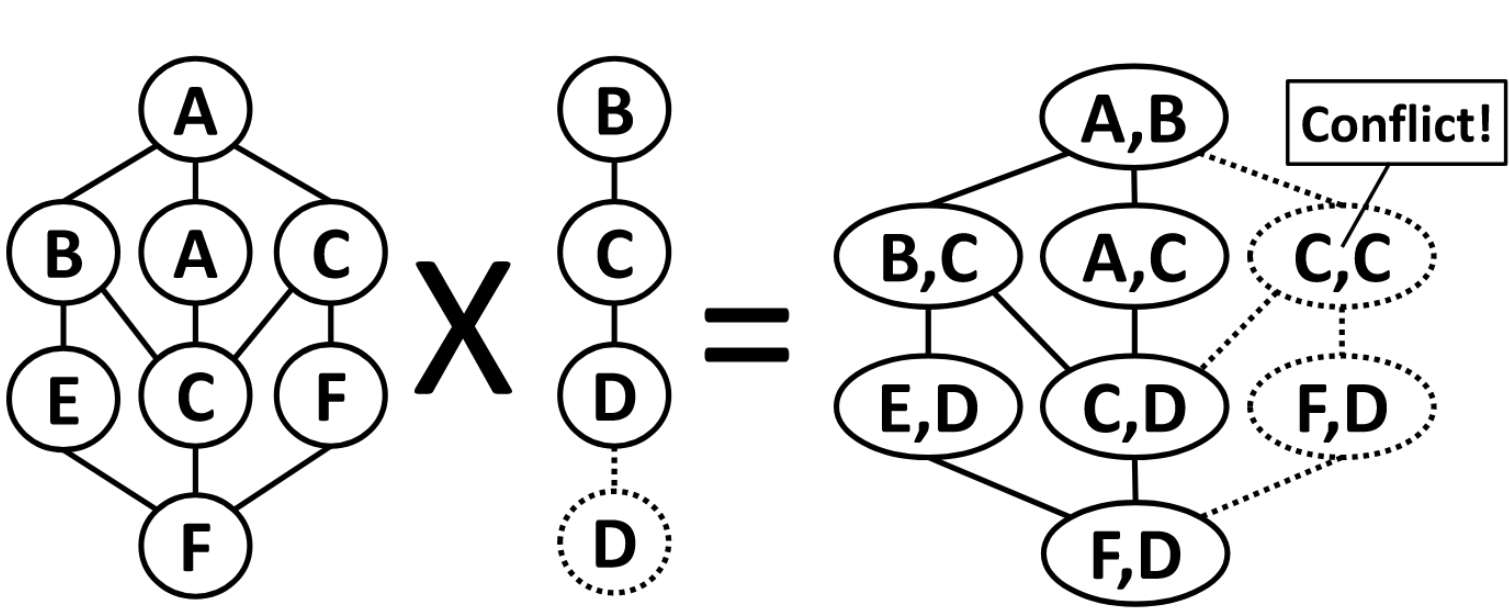
\includegraphics[width=\linewidth]{img/mdds}
			\caption{MDDs for the agents are found and combined.}
			\label{fig:mdds}
		\end{subfigure}
		
		\caption{Example of using ICTS to solve MAPF from \cite{sharon2013}.}
		\label{fig:bottom}
	\end{figure}
	\subsubsection{Bottom-level search}
	Explicitly generating all paths to the goal for agent $a_i$ of cost $c_i$ is expensive: the number of paths is exponential in $c_i$. This is why in the low-level search of ICTS, multi-valued decision diagrams (MDDs) are used to compactly represent all paths per agent. For agent $a_i$ with a target cost $c_i$ (from the cost vector), $MDD_i^{c_i}$ can be generated by a breadth-first search on the $c_i$-steps time-expanded graph starting at $s_i$, followed by a process similar to the standard path reconstruction method used in A* but allowing multiple node parents. Storing the resulting paths in an MDD, which has at most $|V|$ nodes at each timestep or depth, avoids the cost of storing all paths explicitly and facilitates the efficient search of the $k$-agent space of path combinations \cite{sharon2013}.
	
	In Figure \ref{fig:bottom}, a problem with its corresponding ICT is shown, as well as the low-level search of the (solution) node $(3,2)$ using MDDs. The second agent staying at node D after completing the path is also modeled in its MDD to ensure that the place remains blocked.
	
	Subfigure \ref{fig:mdds} illustrates how two or more MDDs can be combined: first, the root nodes are joined; next, the product of the children of both roots is taken and checked for conflicts. In \ref{fig:mdds}, a vertex conflict occurs and therefore this joint child can be removed from the MDD. If a $(B,A)$ node would be generated by the same root, $(A,B)$, this would be an edge conflict and hence $(B,A)$ would also be removed from the joint MDD $MDD_{1,2}^{c_1,c_2}$. In the next layer, the process repeats with multiple parent nodes.
	
	In practice, joint MDDs are not explicitly constructed but instead, a depth-first search is used to search joint MDDs. This has the benefit of finding a path to the bottom of the joint MDD fast if one exists, while not constructing more of the joint MDD than is necessary for finding a solution, which can get large.
	\subsubsection{ICTS with Independence Detection}
	Like other MAPF algorithms, ICTS can be embedded in the Independence Detection (ID) framework introduced by Standley \cite{standley2010}. ID starts by assuming each agent is a group that can be assigned an optimal path independent of other groups. If group paths do conflict, they become one group that is planned together using a MAPF algorithm, in this case, ICTS, until no conflicts between groups occur. The goal of ID is to minimize $k'$, the size of the largest group that has to be planned. Optionally, a conflict avoidance table (CAT) can be maintained for use during the planning of groups. This records the paths planned by other groups and can facilitate tie-breaking in search that minimizes the number of conflicts; the CAT is omitted from Algorithm \ref{id-algo} for brevity but was implemented and used in experiments.
	\begin{algorithm}
		\begin{algorithmic}[1]
			\State \text{Assign each agent to a singleton group}
			\State \text{plan a path for each group}
			\Repeat
			\State \text{simulate execution of all paths until a conflict occurs}
			\State \text{merge two conflicting groups into a single group}
			\State \text{cooperatively plan new group}
			\Until{\text{no conflicts occur}}
			\State $solution\gets\text{paths of all groups combined}$
			\State \textbf{return solution}
		\end{algorithmic}
		\caption{Simple Independence Detection \cite{standley2010}} 
		\label{id-algo}
	\end{algorithm}
	\subsubsection{Pruning in ICTS}
	\label{pruning}
	In addition to ID, three pruning methods can be used to speed up ICTS \cite{sharon2013}, two of which are used in this work. These methods rely on the fact that if no solution exists for any combination of $j$ out of $k$ agents with $j < k$, no solution exists for all $k$ agents. If any such combination is found for a node, there is no need to search the $k$-agent MDD so the next ICT node can be considered. The three pruning methods are as follows.
	\begin{enumerate}
		\item Simple pruning: for all combinations of $j$ out of $k$ agents, the $j$-agent MDD is searched using DFS for a solution.
		\item Enhanced pruning: for all combinations of $j$ out of $k$ agents, the $j$-agent MDD is searched using BFS and when children are generated, for each agent, all children that do not appear in any unified node are removed from the MDD. In \ref{fig:mdds}, the $C$ node of $MDD_1$ would be removed as it cannot be unified with any node of $MDD_2$ at that level.
		\item Repeated enhanced pruning: the enhanced pruning procedure is repeated until a fixed point is reached, which is when no child node is removed from any of the agent MDDs in an iteration. This was not used in this work. 
	\end{enumerate}
	The full ICTS algorithm including a pruning step as described above is given by Algorithm \ref{icts-algo}. It is reproduced from \cite{sharon2013} for completeness. In this work, triple-pruning ($j=3$) was used and enhanced triple-pruning was taken as a baseline, as this often outperforms other variants \cite{sharon2013}.
	\begin{algorithm}
		\begin{algorithmic}[1]
			\Procedure{ICT-search}{MAPF instance}
			\State \text{Construct ICT root}
			\ForAll{\text{ICT nodes }$(c_1,\ldots,c_k)$\text{ in breadth-first order }} 
			\ForAll{\text{agents} $a_i$} 
			\text{Construct} $MDD_i^{c_i}$
			\EndFor
			\ForAll{$j$-\text{agent combinations} $(i_1,\ldots,i_j)$} 
			\State \text{Run node-pruning procedure with MDDs }$MDD_{i_1}^{c_{i_1}},\ldots,MDD_{i_j}^{c_{i_j}}$
			\If{\text{no solution was found for a combination in pruning}}
			\State \textbf{Break}\text{ and continue with next ICT node}
			\EndIf
			\EndFor
			\State \text{Search }$k$\text{-agent MDD space}
			\If{\text{solution was found}}
			\State \textbf{return solution}
			\EndIf
			\EndFor
			
			\EndProcedure
		\end{algorithmic}
		\caption{Increasing Cost Tree Search}
		\label{icts-algo}
	\end{algorithm}
	\subsection{Exhaustive ICTS}
	\label{exhaustive}
	For $K$ teams $t_1,\ldots,t_K$ of size $k_i$, there are in total $M = \prod_{i} k_i!$ matchings from team agents to team goals. These matchings can be enumerated by representing each permutation $p_i$ of goals for each team $t_i$ as an integer $n \in \{1,\ldots,k_i!\}$. Using such numbering, each $e \in \{1,\ldots,k_1!\} \times \cdots \times \{1,\ldots,k_K!\}$ corresponds to a unique combination of permutations and can be mapped to a matching $m$ assuming some fixed ordering of agents within each team. Let $C_1$ through $C_M$ denote the optimal SIC costs of each MAPF instance corresponding to the MAPFM instance, with $C_m = \infty$ for infeasible matching $m$. In order to find the optimal solution, $m$ with lowest $C_m$ has to be found, which requires all $M$ matchings to be solved or found to be infeasible, meaning that $\mathcal{O}(M)$ MAPF instances have to be solved. 
	\subsubsection{Bounded search}
	Once a solution is found for a matching $m$ with cost $C_m$, this can be used in the next search as an (exclusive) upper-bound $B$ for the SIC of nodes that have to be searched. Formally, let $B_0 = \infty$ represent the initial SIC bound of the ICT search. After solving each $m$ with solution cost $C_m$, let $B_{m+1} = \min(B_m,C_m)$. By successively updating $B$ in this manner, as more matchings are solved, the effort needed to solve the remaining matchings can be expected to be reduced significantly. With $C_m$ denoting the optimal SIC for matching $m$, this effort can be expressed as	
	\[\Delta_{m,\text{bounded}} = \min(B_m,C_m) - C^*_m = B_{m+1} - C^*_m\]
	This is proportional to the effort due to the complexity of the ICTS search for matching $m$, $\mathcal{O}(k^{\Delta_{m,\text{bounded}}})$.
	If $B_m \leq C^*_m$, only the root node will be generated to determine this so $\Delta_{m,\text{bounded}} = 0$.
	Using this, the number of ICT nodes searched in total becomes $\mathcal{O}(\sum_m k^{\Delta_{m,\text{bounded}}})$.
	\subsubsection{Ordered enumeration}
	\label{ordered-enum}
	To reduce the total effort, the matchings $m$ can instead be enumerated and solved in increasing order of $C^*_m$. In this case, the effort per matching is monotonically non-increasing by Property \ref{monotonicity}. This induces a case in which this enumeration minimizes the number of nodes searched in total (Property \ref{cond-monoton-optim}). However, cases in which $\Delta_m$ of the first $m$'s searched is much higher could also be constructed, in which case this approach might cause more nodes to be processed in total than alternative methods. Therefore, this ordered enumeration remains a heuristic improvement that works well in practice, as shown in Section \ref{experiments}.
	
	\begin{property}[Monotonicity]
		\label{monotonicity}
		In bounded exhaustive search using ICTS, solving the matchings in increasing order of root SIC makes the effort $\Delta_{m,\text{bounded}}$ monotonically non-increasing as a function of $m$.
	\end{property}
	\begin{proof}
		Due to the order of matchings for successive matchings $m,m+t$ for some $t\geq 1$, $C^*_{m} \leq C^*_{m+t}$. By definition, $B_{m+2} = \min(B_{m+1},C_{m+1})$ meaning that $B_{m+2} \leq B_{m + 1}$ so transitively $B_{m+t+1} \leq B_{m+1}$. Therefore
		\[B_{m+t+1} - C^*_{m+t}\leq B_{m+1} - C^*_m\implies \Delta_{m+t,\text{bounded}} \leq \Delta_{m,\text{bounded}}\]
	\end{proof}
	\begin{property}[Conditional optimality]
		\label{cond-monoton-optim}
		Assuming that $\Delta_m$, the unbounded effort, is monotonically non-decreasing as a function of $m$ (with $m$ in increasing order of $C^*_m$), ordered enumeration minimizes the total number of nodes searched across matchings.
	\end{property}
	\subsubsection{Approximate ordered enumeration}
	In the implementation of exhaustive ICTS, matchings are enumerated by taking the product of goal permutation indices as described above so they are not enumerated in increasing order of root SIC. To achieve this ordering, matchings would have to be exhaustively enumerated and stored in memory before being sorted. Storing all matchings requires $\mathcal{O}(M)$ memory which was found to be more problematic in practice than the time complexity of the sorting, $\mathcal{O}(M\log(M))$. This is why in implementation, ordered enumeration is approximated using a priority queue that maintains a subset of matchings of a fixed size $M_{pq}$.\footnote{$M_{pq} = 10000$ was used in implementation but this could be much increased at the cost of memory.} Algorithm \ref{pq-algo} outlines the procedure.
	
	
	%Using the 
	%To generate matchings 
	%In the implementation of exhaustive matching, the algorithm used to generate matchings
	%The algorithm for generating 
	%In the implementation of ordered enumeration as described above, matchings are not generated in increasing order of root SIC. As a result, to achieve this ordering, matchings have to be exhaustively enumerated and stored in memory to be sorted. This requires $\mathcal{O}(M)$ memory which was found to be more problematic in practice than the time complexity of the sorting, $\mathcal{O}(M\log(M))$.
	
	%In practice, it is difficult to enumerate all matchings in increasing order of root SIC. Finding a lowest SIC $m$ reduces to the assignment problem that can be solved using the Hungarian algorithm \cite{kuhn55} in polynomial time; 
	%[TODO]
	
	
	%however, to the knowledge of the author, no algorithm exists to more generally compute the $i$'th matching in increasing order of $C^*_m$ (assuming some fixed tie-breaking). This means that matchings have to be exhaustively enumerated and stored in memory to sort them, but this requires $\mathcal{O}(M)$ memory which was found to be more problematic in practice than the time complexity of the sorting, $\mathcal{O}(M\log(M))$.
	
	\begin{algorithm}
		\begin{algorithmic}[1]
			\State \text{Fill PQ with }$\min(M,M_{pq})$\text{ matchings}
			\State $B \gets \infty$
			\State $solution \gets none$
			\Repeat
			\State $m\gets\text{Take matching with lowest SIC from PQ}$
			\State $solution_m$ \text{with cost} $C_m\gets$\text{Solve $m$ with upper-bound }$B$ 
			\If{\text{$C_m < B$}}
			\State $B\gets C_m$
			\State $solution \gets solution_m$
			\EndIf
			\State $B\gets\min(B,C_m)$
			\If{\text{there is an unsolved matching }$m_{new}$\text{ not in }$PQ$}
			\State \text{Compute root SIC and insert }$m_{new}$\text{into PQ}
			\EndIf
			\Until{\text{PQ is empty}}
			\Return $solution$
		\end{algorithmic}
		\caption{Approximate ordered exhaustive ICTS} 
		\label{pq-algo}
	\end{algorithm}
	
	\subsection{ICTS-m}
	ICTS with Matching (ICTS-m) generalizes ICTS to optimally solve MAPFM instances. Few changes to ICTS were necessary to accommodate for matching in this increasing cost tree scheme. Specifically, the ICT root generation and the MDD generation as described in Subsection \ref{icts} had to be changed.
	\subsubsection{Root generation for matching}
	Given a team $t_i$ of size $k_i$, for any agent $a_j^i$ there are $k_i$ costs $c_j(1),c_j(2),\ldots,c_j(k_i)$ for shortest paths from $s_j^i$ to each goal $g_k^i$. Making no assumptions about what goals other agents in $t_i$ are assigned to, it could be that in the optimal solution $a_j^i$ is assigned to a goal $g_{m}^i$ with path cost $c^*_j = c_j(m)$ such that $c_j(m) = \min_{n\in\{0,\ldots,k_i\}} c_j(n)$. Therefore, to guarantee optimality, this minimal cost to any matching goal has to take the place of the shortest path cost from the original ICTS root. Intuitively, the sum of individual costs of this root is highly optimistic, particularly if the teams are large. This is because often, agents will not move to their closest matching goal in an optimal solution, even without considering conflicts (see \ref{pathology}).
	
	\subsubsection{MDD generation for matching}
	To generate MDDs for MAPFM, each agent also has to consider not one goal but all matching goals. To do this, the MDD construction following the breadth-first search has to be changed: each goal becomes an endpoint from which paths to the start node are traced, resulting in an MDD with one start node and one or more terminal nodes.
	\begin{wrapfigure}{R}{.35\textwidth}
		\vspace{-10pt}
		\centering
		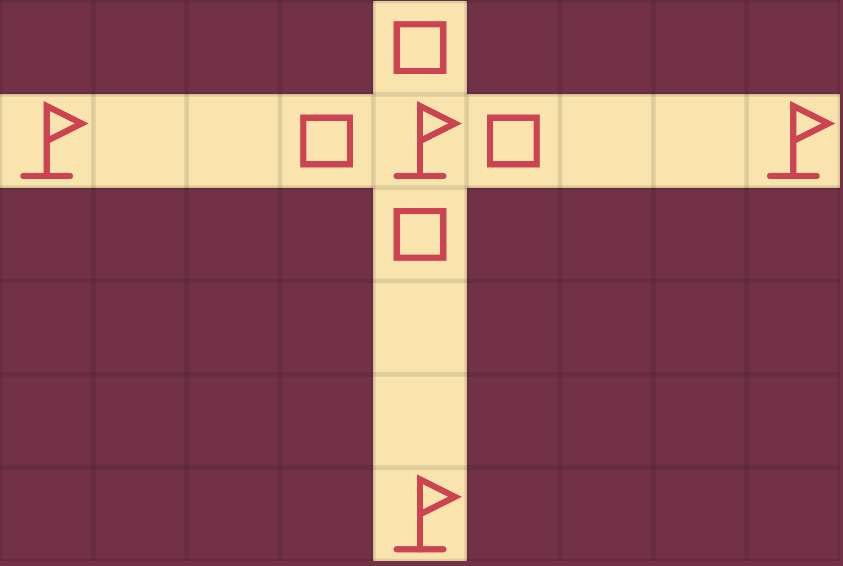
\includegraphics[width=\linewidth]{img/path}
		\caption{Pathological case for ICTS-m. The squares represent agents and the flags represent goals.}
		\label{fig:path}
		\vspace{-10pt}
	\end{wrapfigure}
	\subsubsection{Pathological case}
	\label{pathology}
	As a consequence of the $\min$ operation in the root definition, a pathological case can be derived. Consider a team of 4 agents $a_1^1$ through $a_4^1$. Let them be arranged in a configuration as depicted in Figure \ref{fig:path}. All four agents match the color of the center goal and hence for each $i$, $c^*_i = 1$, so that the root is $(1,1,1,1)$ with SIC $4$. The optimal solution however is $(1,3,3,3)$ with SIC $10$ numbering the agents clockwise, meaning that $\Delta = 6$. It can be seen that instances of this form with arbitrarily large $\Delta$ can be constructed. As ICTS-m being a generalization of ICTS is $\mathcal{O}(k^\Delta)$, even just extending the limbs of the instance to yield an ICT root of $(1,9,9,9)$ with $\Delta = 24$ will result in an unfathomably large number of nodes being evaluated assuming no pruning or other modifications to the base algorithm.
	%\subsubsection{Inverted MDD search}
	%The uniqueness of goals guarantees the existence of a goal node without vertex conflicts in searching MDDs in MAPF. In MAPFM, this is not the case and causes joint MDDs to be searched fully without finding a result. In addition, even if there exists a goal node, many of the paths represented by the joint MDD lead to conflicting maximal-depth nodes.
	
	%To avoid this, the MDD search could be changed to start at the maximal depth and search for a way towards the start node, which by start uniqueness remains without vertex conflicts.
	%Two strategies could be used to avoid this: firstly, the MDD search could be changed to start at the maximal depth and search for a way towards the start (which by start uniqueness is always non-conflicting); secondly, a bipartite matching algorithm could be employed to see if any matching exists between agents and goals they can reach. An advantage of the former strategy is that it will, in particular with larger team sizes, reduce the number of maximal depth nodes drastically, so that the subsequent search is from few nodes to one goal. By only running a matching algorithm to skip regular MDD search, there is no such reduction so from one starting position paths will be searched to potentially an exponential number of goal nodes, of which many will end up being illegal. 
	%[TODO: just focus on explaining why inverted MDD search was/could be used to solve this? Or just toss this out for lack of time/space. Why didn't I come up with this idea earlier...]
	\subsection{Optimizations}
	To improve both types of algorithms, some optimizations were found that can be used to speed up the search.
	\subsubsection{Bounds in ID}
	The information gained about solution costs of independent groups can be used to establish a lower bound on solution SIC as per Property \ref{property:id-lower}. In bounded search, the upper bound can be further constrained by Property \ref{property:id-upper}.
	\begin{property}[Lower bound]
		When merging groups $g_i,g_j$ with solution costs $C_i,C_j$ to yield group $g_k$, for any solution for this group with cost $C_k$
		\[C_k\geq C_i + C_j\]
		\label{property:id-lower}
	\end{property}
	\begin{proof}
		Assume there would be a solution with $C_k < C_i + C_j$. Taking $C_k^i$ to denote the SIC of agents that used to make up $g_i$ in the solution to $g_k$, without loss of generality $C_k^i < C_i$, which contradicts the optimality of the solution with cost $C_i$ for $g_i$ independent of $g_j$.
	\end{proof}
	\begin{property}[Reduced upper bound]
		In bounded exhaustive search, the sum of costs of groups not being merged can be subtracted from bound $B$ without losing optimality.
		\label{property:id-upper}
	\end{property}
	\subsubsection{Child pruning}
	In the original ICTS formulation all $k$-children are generated in every case because pruning only controls skipping the low-level search, assumed to be the most expensive operation. However, in simple pruning in any case, when there is a conflict between two or more agents at a given ICT node $(c_1,\ldots,c_k)$, in any solution, one or more of the path costs corresponding to these conflicting agents will have to be incremented. This can be exploited by pruning the node's children that do not correspond to the conflicting agents, of which there are often just 2 or 3, drastically improving the (average) branching factor as $k$ increases. By Property \ref{property:ec-incompat}, child pruning is not compatible with enhanced pruning.
	\begin{property}[Incompatibility with enhanced pruning]
		Enhanced pruning combined with child pruning is suboptimal due to the \textit{cascading effect} described in \cite{sharon2013}.
		\label{property:ec-incompat}
	\end{property}
	
	\begin{figure}[H]
		\centering
		\begin{subfigure}{0.40\textwidth}
			\centering
			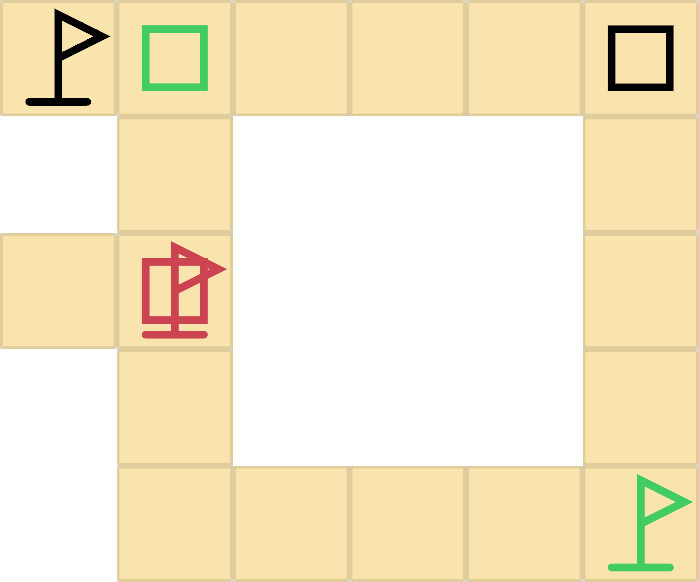
\includegraphics[width=\linewidth]{img/counter-example-ep-2}
			\caption{Counter-example instance.}
			\label{fig:counter-example:a}
		\end{subfigure}
		\begin{subfigure}{0.49\textwidth}
			\centering
			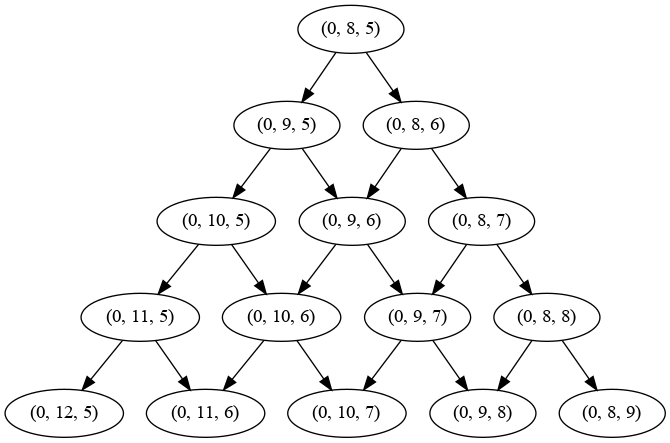
\includegraphics[width=\linewidth]{img/counter-example-tree}
			\caption{Pruned ICT that is traversed.}
			\label{fig:counter-example:b}
		\end{subfigure}
		\caption{Counter-example for enhanced pruning combined with child pruning. If the black and green agent pair is considered last, an ICT is traversed while solving the instance that does not contain an optimal solution.}
		\label{fig:counter-example}
	\end{figure}
	\begin{proof}
		Consider Figure \ref{fig:counter-example:a} with a red agent $r$, green agent $g$ and black agent $b$. It can be seen that $(3,8,5)$ with SIC $16$ is an optimal solution for this instance, which corresponds to $r$ moving aside, allowing $g$ to pass.  Say enhanced pruning with pairs is applied to these three agents at $(c^*_r,c^*_g,c^*_b) = (0,8,5)$. Let the enhanced pruning order be $(r,g)$, $(r,b)$, $(g,b)$ without loss of generality. $(r,g)$ is solvable but will leave for $g$ out of the two paths of length $8$ only the clock-wise path. $(r,b)$ will not change either MDD in this node. When $(g,b)$ is evaluated, it is found that the remaining clockwise path for $g$ and $b$'s path are incompatible (edge conflict) so $(0,9,5)$ and $(0,8,6)$ are generated. By repeating this order of enhanced pruning with child pruning, the ICT shown in \ref{fig:counter-example:b} is traversed. None of the nodes with SIC 16 in this ICT is a solution, meaning that enhanced pruning combined with child pruning will return a suboptimal solution to the instance in \ref{fig:counter-example:a}, making this pruning strategy suboptimal.
	\end{proof}
	
	\section{Experimental Results}
	\label{experiments}
	To compare the algorithms and variants described above with each other and with alternative MAPFM algorithms, two types of experiments were performed. In the first, ICTS-based algorithms discussed in this work are compared; in the second, the approximate ordered enumeration variant is compared to other algorithms for MAPFM \cite{donszelmann2021,baauw2021,jong2021,bruin2021}. The data for the second experiment originates in \cite{donszelmann2021}.  In both experiments, there are three variables: the number of agents, the fraction of blocked grid tiles and the number of teams. The values measured are the fraction of instances solved and the average run time per instance. In the latter, the recorded run times converge to the 120s timeout used as fewer instances are solved; therefore, while the times are included for completeness at the end of this work (Figure \ref{fig:i-times} and \ref{fig:r-times} for experiments 1 and 2), only the fraction of instances solved is used in the analysis of results.
	%\newgeometry{left=1cm,right=1cm,top=0.1cm,bottom=0.1cm}
	\begin{figure*}[t]
		\centering
		\begin{subfigure}{\graphwidth}
			\centering
			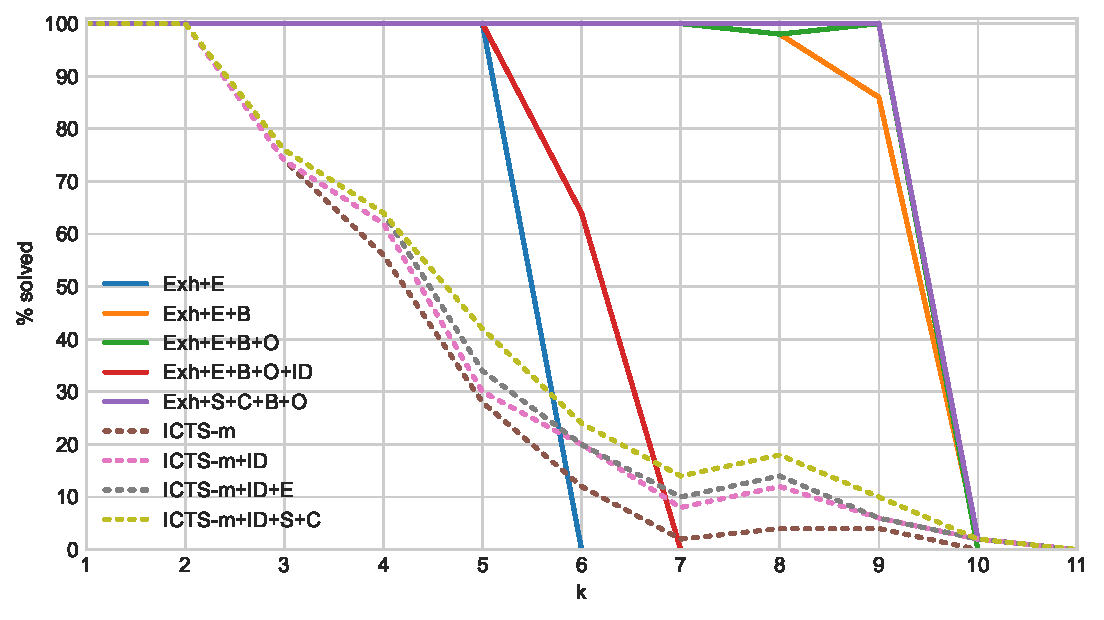
\includegraphics[width=\linewidth]{img/results/icts-comparison/25-1-p}
			\caption{25\% wall, one team.}
			\label{fig:i-25-1-p}
		\end{subfigure}
		\begin{subfigure}{\graphwidth}
			\centering
			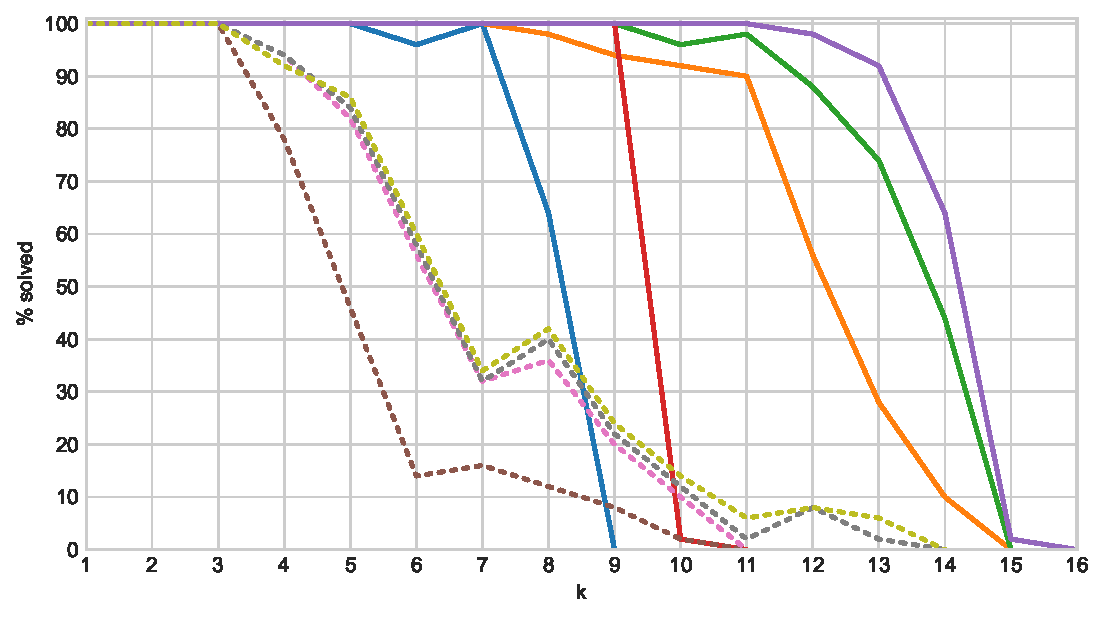
\includegraphics[width=\linewidth]{img/results/icts-comparison/25-3-p}
			\caption{25\% wall, three teams.}
			\label{fig:i-25-3-p}
		\end{subfigure}
		\begin{subfigure}{\graphwidth}
			\centering
			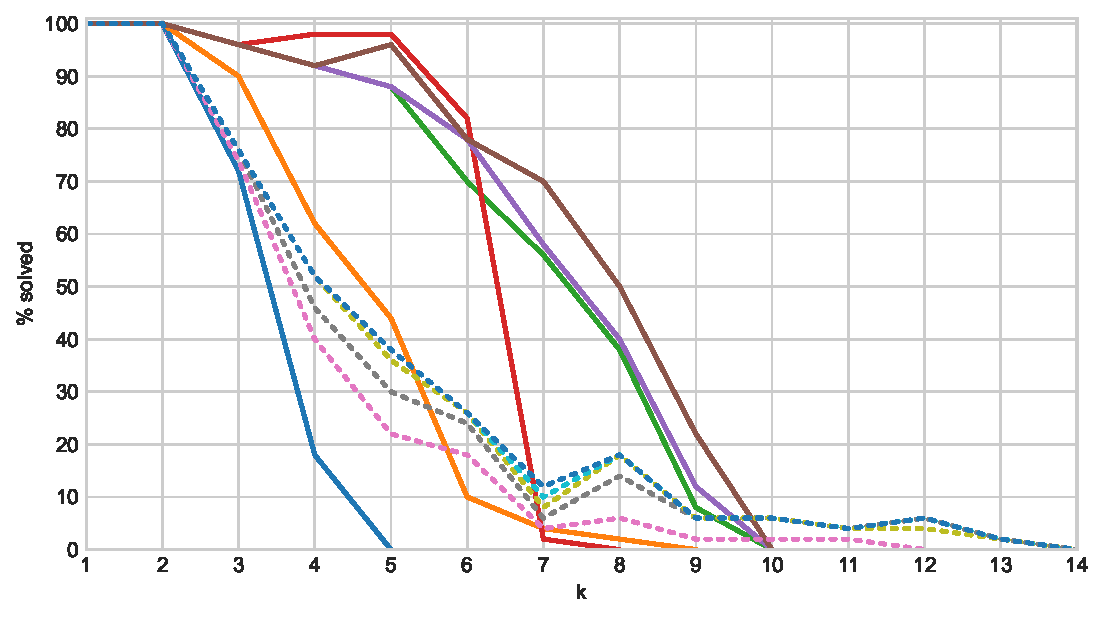
\includegraphics[width=\linewidth]{img/results/icts-comparison/75-1-p}
			\caption{75\% wall, one team.}
			\label{fig:i-75-1-p}
		\end{subfigure}
		\begin{subfigure}{\graphwidth}
			\centering
			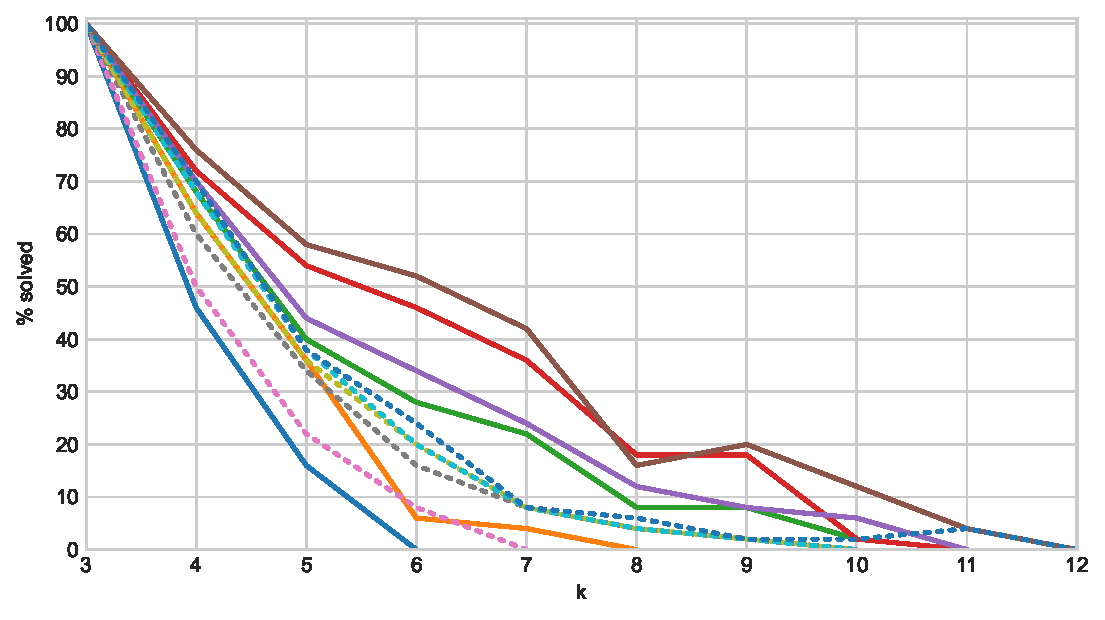
\includegraphics[width=\linewidth]{img/results/icts-comparison/75-3-p}
			\caption{75\% wall, three teams.}
			\label{fig:i-75-3-p}
		\end{subfigure}
		\caption{Fraction solved out of 50 instances by different ICTS-based algorithms.}
		\label{fig:i-probs}
	\end{figure*}
	\begin{figure*}[b]
		\centering
		\begin{subfigure}{\graphwidth}
			\centering
			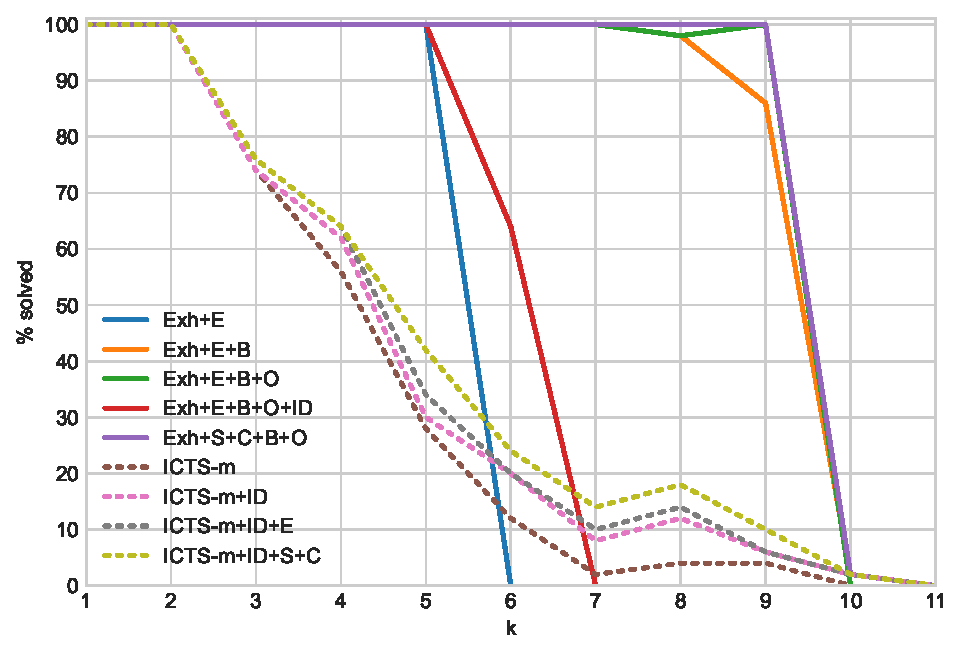
\includegraphics[width=\linewidth]{img/results/relative-comparison/25-1-p}
			\caption{25\% wall, one team.}
			\label{fig:r-25-1-p}
		\end{subfigure}
		\begin{subfigure}{\graphwidth}
			\centering
			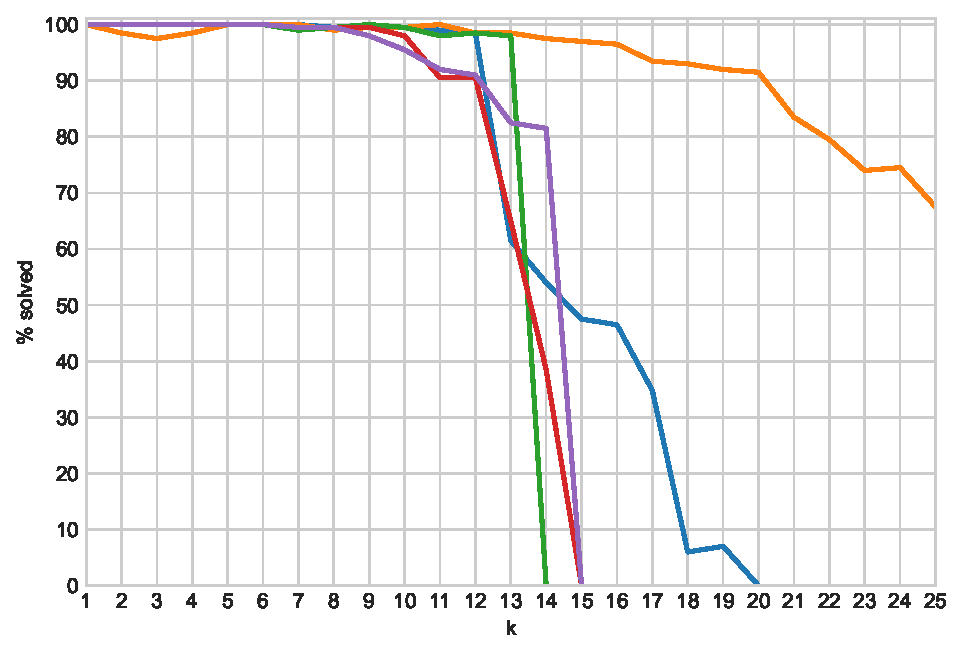
\includegraphics[width=\linewidth]{img/results/relative-comparison/25-3-p}
			\caption{25\% wall, three teams.}
			\label{fig:r-25-3-p}
		\end{subfigure}
		\begin{subfigure}{\graphwidth}
			\centering
			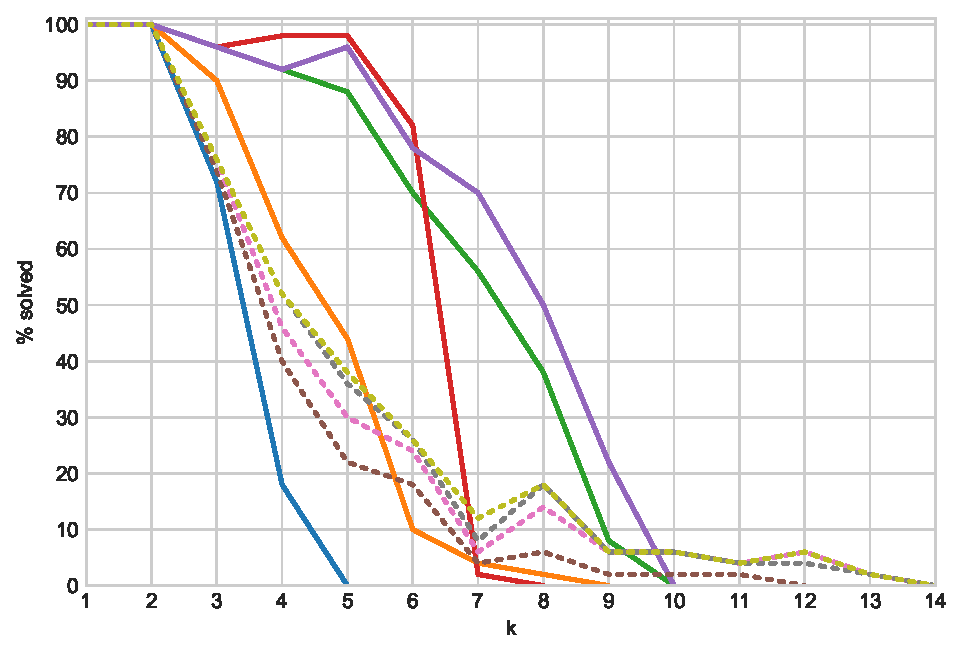
\includegraphics[width=\linewidth]{img/results/relative-comparison/75-1-p}
			\caption{75\% wall, one team.}
			\label{fig:r-75-1-p}
		\end{subfigure}
		\begin{subfigure}{\graphwidth}
			\centering
			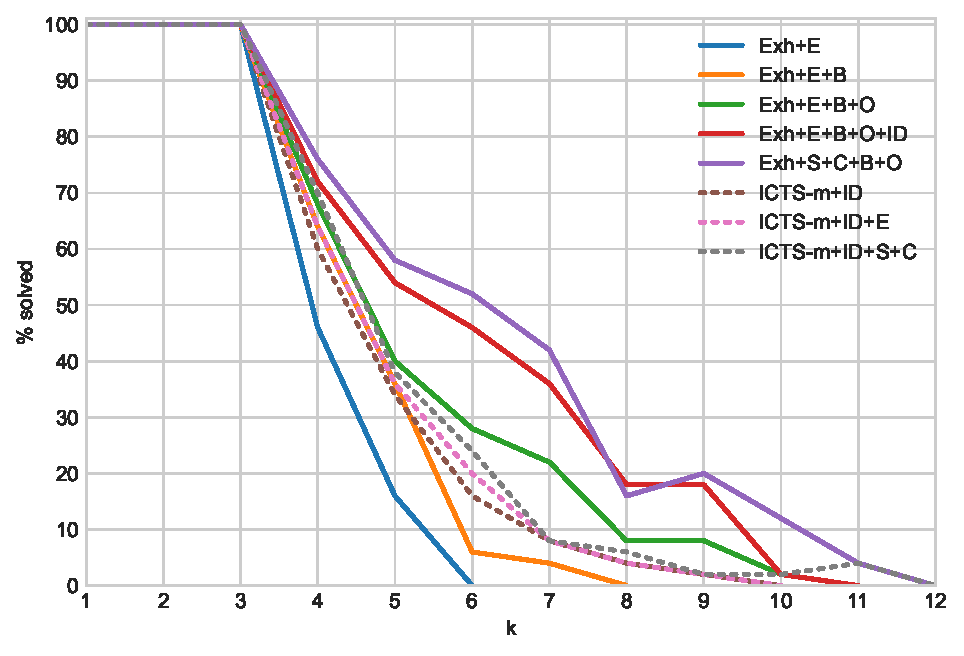
\includegraphics[width=\linewidth]{img/results/relative-comparison/75-3-p}
			\caption{75\% wall, three teams.}
			\label{fig:r-75-3-p}
		\end{subfigure}
		\caption{Fraction solved out of 200 instances by MAPFM algorithms.}
		\label{fig:r-probs}
	\end{figure*}
	
	\restoregeometry
	\subsection{Experimental setup}
	Because MAPFM lies on the fringe of pathfinding research, no standard benchmark exists. For MAPF, the Moving AI benchmarks \cite{sturtevant2012} are often used and potentially a new MAPFM standard benchmark could be defined by generating suitable team-partitions of agents for these MAPF instances; however, it was noticed that optimally solving even small MAPFM instances with comparatively few agents and short distances to goals was already a challenge computationally. This observation informed the creation of a map generator by the author of \cite{bruin2021} with various parameters. 
	
	%Using this generator, MAPFM instances situated on 20x20 grids with obstacles were generated by varying three variables: the number of agents; the fraction of blocked grid tiles; the number of teams. 
	
	Using this map generator, two types of 20x20 grids similar to the random maps in \cite{sturtevant2012} were generated:
	
	\begin{enumerate}
		\item 25\% wall: a grid with 25\% of tiles being obstacles.
		\item 75\% wall: a grid with 75\% of tiles being obstacles. 
	\end{enumerate}
	For each of these types, instances were generated with between $1$ and $25$ agents either all in the same team or evenly partitioned into three teams. For each combination of map-type, number of teams and number of agents, 200 instances were generated. In scenarios with three teams, instances with $k < 3$ were not used. When solving the instances, for each combination of map-type and number of teams, the number of agents was increased until 0\% of instances could be solved within a timeout of 120s, at which point no more data was recorded for greater numbers of agents. This approach is similar to the method described in \cite{stern2019}.
	
	% For each of these types, maps were generated with $K = 1$ and $K = 3$ and $k$ from $K$ to $25$. When solving the instances, for each combination of map-type and $K$, $k$ was increased until 0\% of instances could be solved within a timeout of 120s, at which point no more data was recorded for larger values of $k$. This approach is similar to the method described in \cite{stern2019}.
	
	%In varying the number of obstacles and the number of agents, this setup is similar to those used in the MAPF literature \cite{stern2019}.
	
	% In varying the number of obstacles and the number of agents, the comparison is similar to those used in the MAPF literature \cite{stern2019}. 
	
	
	
	
	
	%The purpose of 
	
	%Although the maps with one team are equivalent to anonymous MAPF instances
	
	
	%While progressively increasing the number of agents is common in MAPF benchmarks
	
	
	
	
	
	The first experiments were performed on a 2.2GHz Intel i7-8750H hexacore with 16GiB of memory. For each setting, a fixed subset of 50 out of 200 instances was used. %Hyperthreading was used in experiments, but because agent-settings were solved in sequence as batches, it is expected that this has affected experimental outcomes equally.
	
	The second experiments comparing the different MAPFM algorithms within the peer group were run on a server with a virtualized Intel Xeon E5-2683 dodecacore operating at 2.0GHz with 8GiB of RAM. All 200 instances were used for each setting.
	
	All algorithms are implemented in Python 3.9 to avoid performance differences as often seen between interpreted versus compiled languages; however, CBM \cite{baauw2021} in experiment 2 does use an SSP solver implemented in C++ as a subroutine. The comparison in this experiment is more coarse-grained as performance differences are sometimes subtle and could potentially be explained by slight implementation optimizations rather than algorithmic properties.
	
	\subsection{Experiment 1: ICTS-based MAPFM algorithms}
	To investigate the relative performance of various algorithms discussed in Section \ref{section:icts-matching}, a selection of both exhaustive and ICTS-m variants was made. Their performance in terms of fraction of problems solved within a timeout of 120s is shown in Figure \ref{fig:i-probs}. The meaning of the abbreviations used in the legend are as follows:
	\begin{itemize}
		\begin{minipage}{0.45\linewidth}
			\item S: Simple pruning
			\item E: Enhanced pruning
			\item C: Child pruning
		\end{minipage}
		\begin{minipage}{0.45\linewidth}
			\item ID: Independence detection
			\item B: Bounded search
			\item O: Approximate ordered enumeration
		\end{minipage}
	\end{itemize}
	Across scenarios, it is seen that typically exhaustive methods outperform ICTS-m algorithms (\ref{fig:i-probs}), with performance being more similar in the maps with 75\% wall. In particular on 75\% wall maps with three teams (\ref{fig:i-75-3-p}), the performance of ICTS-m+ID (and optional pruning) is seen to outperform bounded exhaustive search as $k$ increases, and some of these also manage to solve a small fraction of 75\% maps with one team that exhaustive methods can not within the time-out (\ref{fig:i-75-1-p}).
	
	Between exhaustive variants, with exception of the ID variant, a type of hierarchy can be distinguished, best illustrated by \ref{fig:i-25-3-p}; almost without exception, Exh+S+C+B+O outperforms Exh+E+B+O which outperforms Exh+E+B which in turn outperforms Exh+E. Bounded search outperforms unbounded search as expected, given that the former does as much work as the latter and often less. Approximate ordering outperforming unordered enumeration is not as obvious from a theoretical standpoint, as discussed in \ref{ordered-enum}, and simply indicates that ordered enumeration works well in practice. Simple pruning with child pruning outperforms enhanced pruning but this needs to be qualified. Comparing Exh+S+B+O with Exh+E+B+O shows that part of the difference can be explained by the use of simple pruning instead of enhanced pruning. Nonetheless, in instances with 75\% wall (\ref{fig:i-75-1-p},\ref{fig:i-75-3-p}) there appears to be a real benefit to searching a smaller ICT. Across ICTS-m variants, similar trends can be observed but the differences across pruning strategies are too slight to draw any conclusions from. As discussed in Section \ref{future}, more work is needed to compare simple child pruning with other pruning methods for ICTS.
	
	The benefit of using ID together with ordered enumeration is not clear. Ordered enumeration with ID performs much better in \ref{fig:i-75-3-p}, a setting with more obstacles and more teams, but ordered enumeration without ID on the other hand is superior in an open setting with a single team (\ref{fig:i-25-1-p}). The overhead associated with the various planning and merging steps (see Algorithm \ref{id-algo}) could be the cause of the slowdown observed once $M$ grows large (\ref{fig:i-25-1-p},\ref{fig:i-75-1-p}); once the upper-bound is tightened, ICTs only have to be searched shallowly so there is no point in going through the steps of ID. This explains why no speedup is seen, as between ICTS-m and ICTS-m+ID. Another factor is that if all agents belong to the same team, it is unlikely that there will be a significant benefit to using ID, as agents from the same team planned independently often route to the same goal.
	
	\subsection{Experiment 2: Algorithms for MAPFM}
	From the variants discussed and compared above, the Exh+E+B+O variant was selected for comparison with various other algorithms for MAPFM. This results in the following set of algorithms whose performance is shown in Figure \ref{fig:r-probs}.
	\begin{itemize}
		\begin{minipage}{0.45\linewidth}
			\item ICTS with approximate sorted exhaustive matching (Exh+E+B+O)
			\item A*+ID+OD with matching ID and sorted exhaustive matching \cite{bruin2021}
			\item EPEA* with matching ID and sorted exhaustive matching \cite{jong2021}
		\end{minipage}
		\hspace{1cm}
		\begin{minipage}{0.40\linewidth}
			\item M* with sorted exhaustive matching \cite{donszelmann2021}
			\item CBM adapted to use SIC, using the successive shortest path algorithm (SSP) \cite{goldberg1987} as subroutine for solving teams \cite{baauw2021}.
		\end{minipage}
	\end{itemize}
	With exception of CBM, all methods described use a variant of sorted exhaustive matching. This is because from each family of algorithms one of the best performing algorithms was chosen, which always was such an exhaustive method as opposed to a generalization of the base algorithm to MAPFM (ICTS-m in this work). A*+ID+OD and EPEA* also make use of matching ID, which is ID applied to the MAPFM instance using the respective exhaustive algorithm as MAPFM solver. The initial groups are here the teams, which is why in single team scenarios (Subfigures \ref{fig:r-25-1-p},\ref{fig:r-75-1-p}) matching ID has no effect. Hypothetically, matching ID could explain why both A*+ID+OD and EPEA* outperform the methods using just sorted exhaustive matching in maps with 75\% wall and three teams (\ref{fig:r-75-3-p}).
	
	CBM solving all problems with one team (Figure \ref{fig:r-25-1-p} and \ref{fig:r-75-1-p}), problems equivalent to anonymous MAPF instances, is at first surprising but follows directly from the definition of the CBM method. CBM solves single teams as anonymous MAPF instances in polynomial time, meaning that solving scenarios with a single team reduces to a polynomial-time procedure, namely SSP. Following the results reported in \cite{ma2016}, it is expected that as the number of teams approaches $k$, CBM performance will deteriorate and thus become more similar to the results for exhaustive methods here reported.
	%	Still, some implementations might be more optimized than others so this might be a factor in performance characteristics and in particular in relative performance differences.
	\section{Conclusions and Future work}
	\label{conclusions}
	\label{future}
	The goal of this research was to seek methods for solving MAPFM based on ICTS. In this, the research has succeeded, but the scalability of the algorithms leaves something to be desired. Exhaustive methods, like those discussed in detail in Subsection \ref{exhaustive}, cannot be expected to scale well as teams grow larger due to their complexity, no matter what optimizations are put in place. Nonetheless, as was shown in Section \ref{experiments}, the more advanced exhaustive ICTS algorithms consistently outperform the ICTS-m based algorithms. Compared to the SIC-adaptation of the CBM method \cite{baauw2021}, it was seen that exhaustive methods generally perform relatively poorly if there are fewer teams and fewer obstacles, while being competitive once teams grow smaller and maps become more constrained. Delineating under which conditions exhaustive methods outperform CBM and vice versa is something for further research.
	
	%\section{Future work}
	A key idea for future research to look into is how to exploit the lower-bound on solution SIC that can be found using the Hungarian Algorithm \cite{kuhn55} or similar methods like the JVC algorithm \cite{jonker1987}. This lower-bound could be used in a branch-and-bound \cite{land1960} search of matchings. An algorithm for MAPF could be used at leaf nodes as in exhaustive ICTS; however, solving (small) branches as MAPFM instances using approaches other than branch-and-bound is also a direction to explore. To retain the benefits of ordered enumeration and to potentially allow for a higher degree of bounding, an optimized version \cite{miller1997} of Murty's algorithm \cite{murty1968} for ranking all matchings in increasing order of cost could be taken as a starting point for such a branch-and-bound approach. 
	
	%in which matchings are enumerated in increasing order of SIC  
	
	
	%for MAPFM could be used to solve (small) branches.
	
	%The most straightforward way would be to use an algorithm for MAPF at leaf nodes but algorithms for MAPFM could be used to solve (small) branches. 
	
	%Specifically, 
	
	%By using the Hungarian Algorithm to determine 
	
	%The most straightforward way would be to use an algorithm for MAPF at leaf nodes but algorithms for MAPFM could be used to solve (small) branches. 
	
	Another possibility would be to use the lower-bound on solution SIC to improve ICTS-m by only executing the $k$-agent low-level search for nodes that satisfy this bound. The lower-bounding in ICTS-m could then be further improved by finding the optimal SIC for the anonymous MAPF instance corresponding to each team using an approach similar to those described in \cite{baauw2021}. As long as there is a team that does not meet its bound, branching only on agents within this team is possible without losing optimality. 
	
	A related observation is that the algorithms introduced in this work do not rely on the property of agents and goals having one color. Both exhaustive ICTS and ICTS-m could easily be adapted to support one or more colors (teams) for each agent and goal while still guaranteeing optimality, in contrast to CBM \cite{ma2016} and its SIC adaptation \cite{baauw2021} which specifically use this property to plan single teams in polynomial time. Future research could study the multi-color MAPFM generalization and the application of methods described in this work to that problem. 
	
	Lastly, more experimentation is needed to reach definite conclusions about how simple child pruning compares to existing pruning techniques for ICTS, which could be done by reproducing the ICTS pruning experiments reported in \cite{sharon2013} extended with simple child pruning variants. 
	
	%Given that simple pruning is somewhat cheap computationally, it might also be possible to prune the child generation using simple child pruning but still use enhanced pruning to decide whether to execute $k$-agent low-level search, combining the benefits of searching a smaller ICT and performing fewer $k$-agent searches.
	
	\section{Reproducibility}
	The implementation of the ICTS-based algorithms described in this work is publicly available online in the form of a Github repository.\footnote{\url{https://github.com/tbvanderwoude/icts-m}} Included is also code for benchmarking different configurations of the ICTS solver and the instances that were used in the benchmarks reported above. The benchmarks and instances used in the relative comparison of MAPFM algorithms are also available in the code and data repository of \cite{donszelmann2021}.\footnote{\url{https://github.com/jonay2000/research-project}}
	
	\printbibliography
	\newpage
	\begin{figure*}[t]
		\centering
		\begin{subfigure}{\graphwidth}
			\centering
			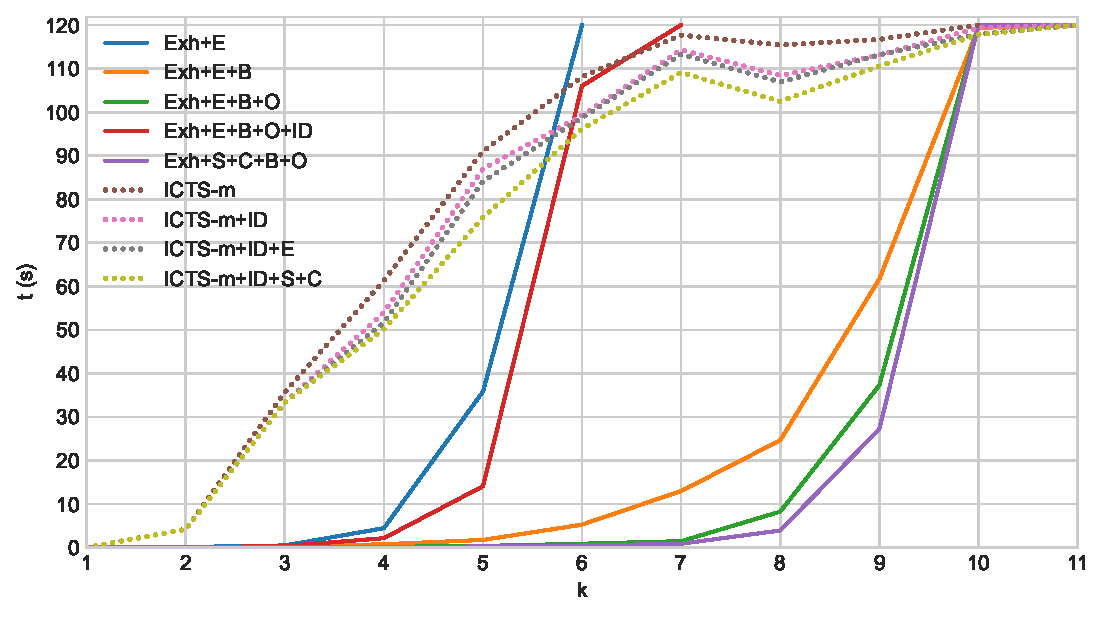
\includegraphics[width=\linewidth]{img/results/icts-comparison/25-1}
			\caption{25\% wall, one team.}
			\label{fig:i-25-1}
		\end{subfigure}
		\begin{subfigure}{\graphwidth}
			\centering
			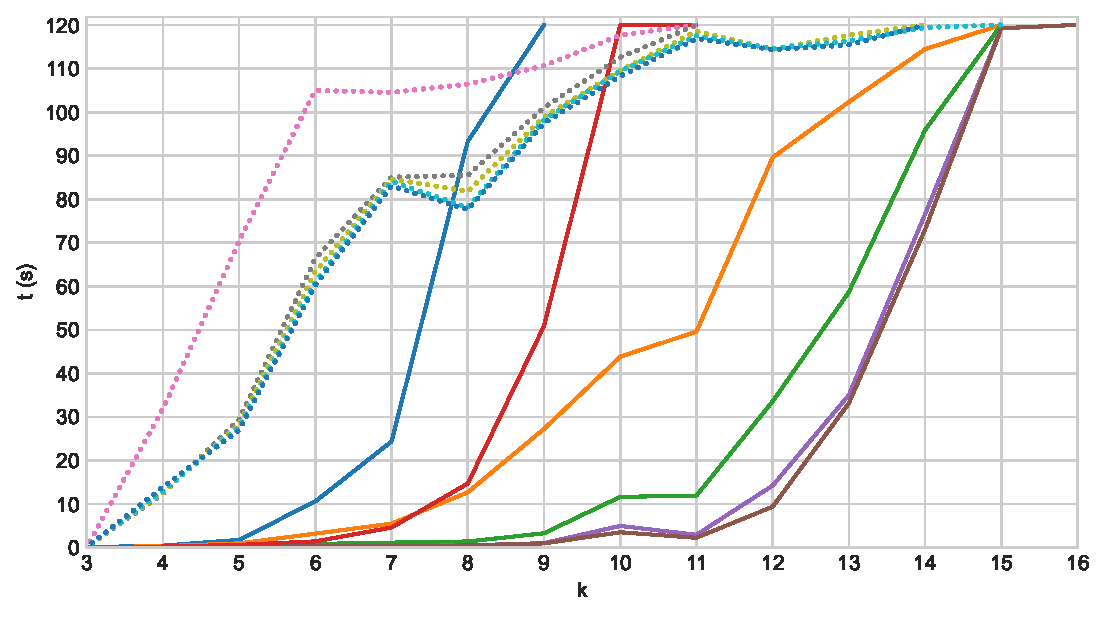
\includegraphics[width=\linewidth]{img/results/icts-comparison/25-3}
			\caption{25\% wall, three teams.}
			\label{fig:i-25-3}
		\end{subfigure}
		\begin{subfigure}{\graphwidth}
			\centering
			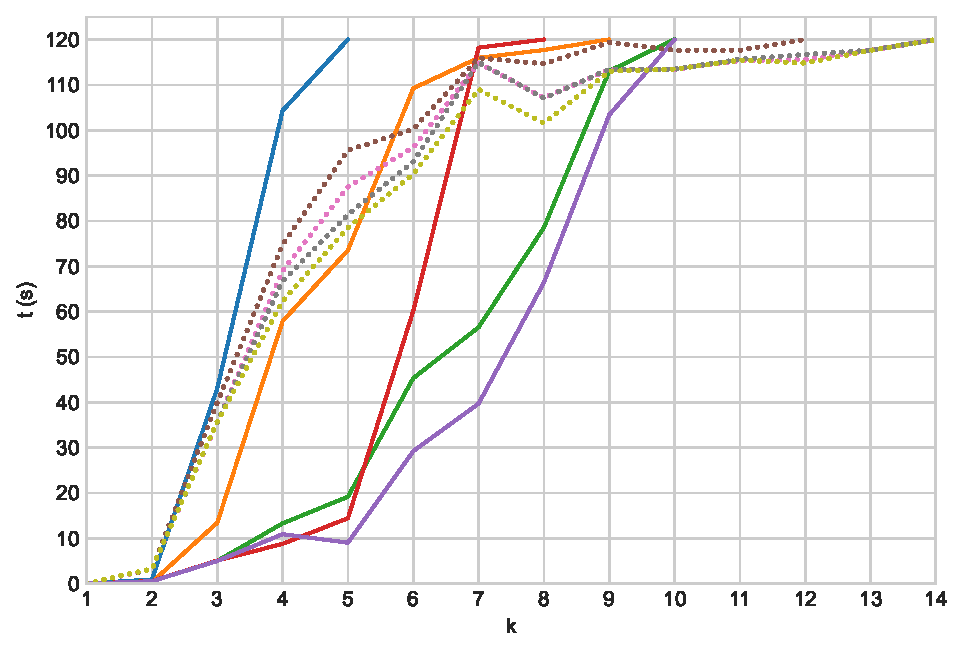
\includegraphics[width=\linewidth]{img/results/icts-comparison/75-1}
			\caption{75\% wall, one team.}
			\label{fig:i-75-1}
		\end{subfigure}
		\begin{subfigure}{\graphwidth}
			\centering
			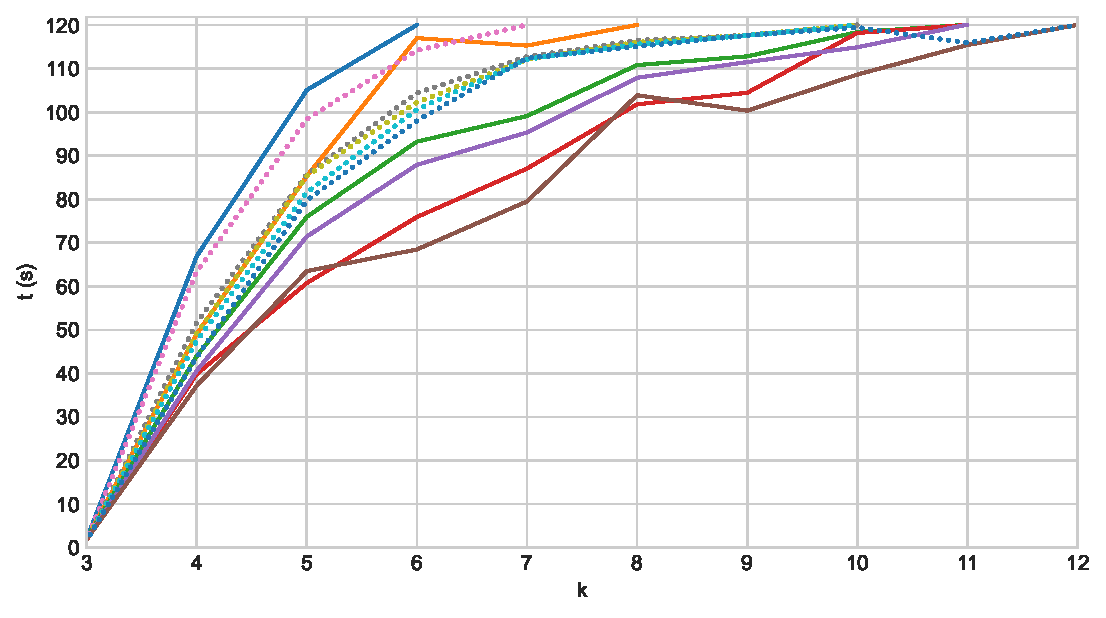
\includegraphics[width=\linewidth]{img/results/icts-comparison/75-3}
			\caption{75\% wall, three teams.}
			\label{fig:i-75-3}
		\end{subfigure}
		\caption{Average solving time of different ICTS-based algorithms with a timeout of 120s.}
		\label{fig:i-times}
	\end{figure*}
	\begin{figure*}[b]
		\centering
		\begin{subfigure}{\graphwidth}
			\centering
			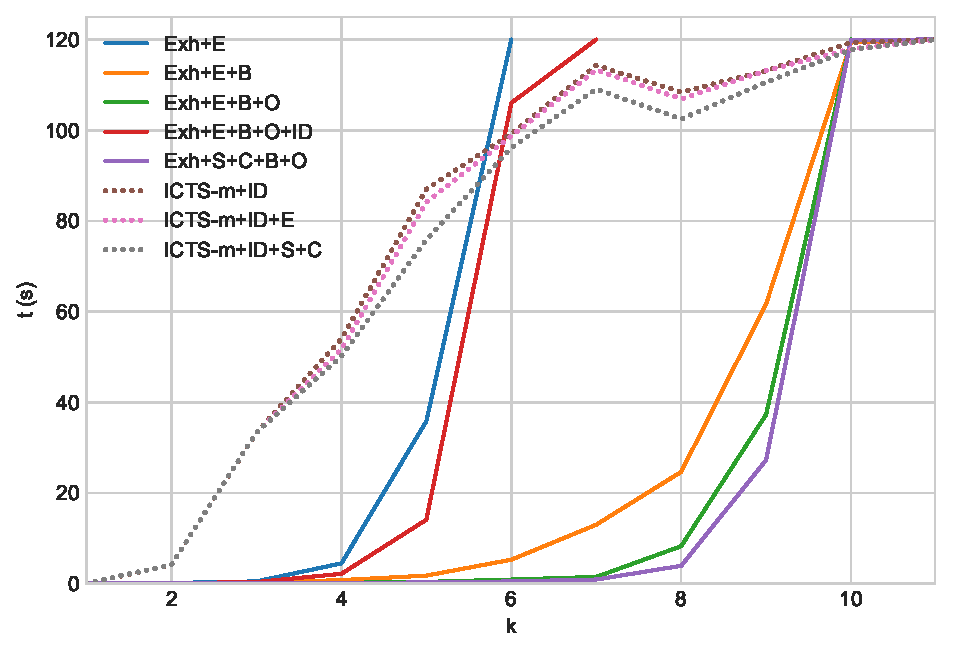
\includegraphics[width=\linewidth]{img/results/relative-comparison/25-1}
			\caption{25\% wall, one team}
			\label{fig:r-25-1}
		\end{subfigure}
		\begin{subfigure}{\graphwidth}
			\centering
			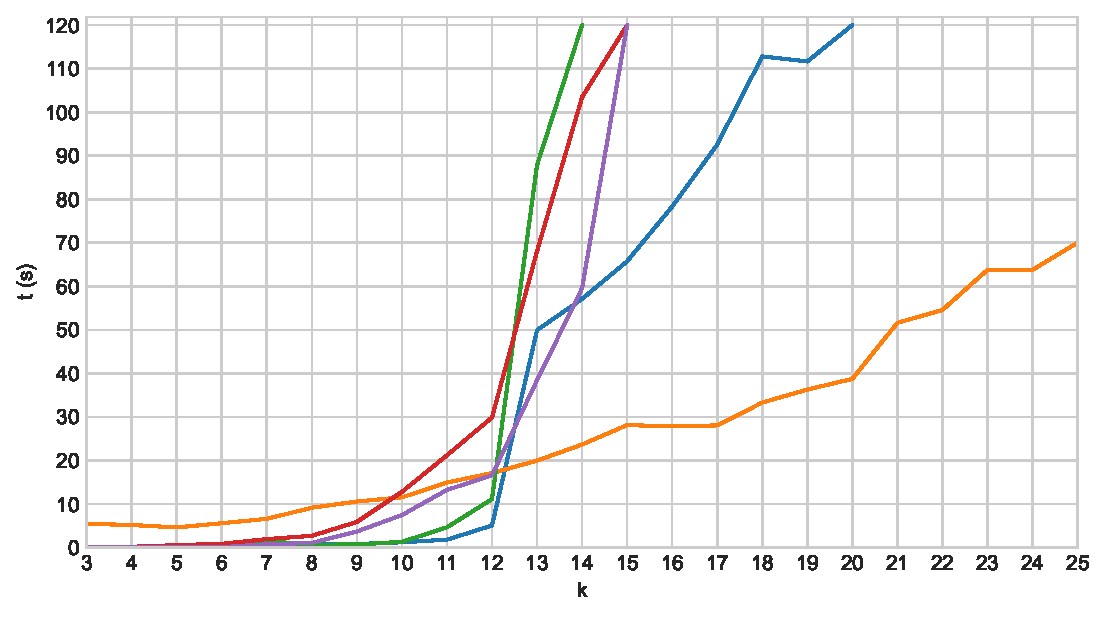
\includegraphics[width=\linewidth]{img/results/relative-comparison/25-3}
			\caption{25\% wall, three teams}
			\label{fig:r-25-3}
		\end{subfigure}
		\begin{subfigure}{\graphwidth}
			\centering
			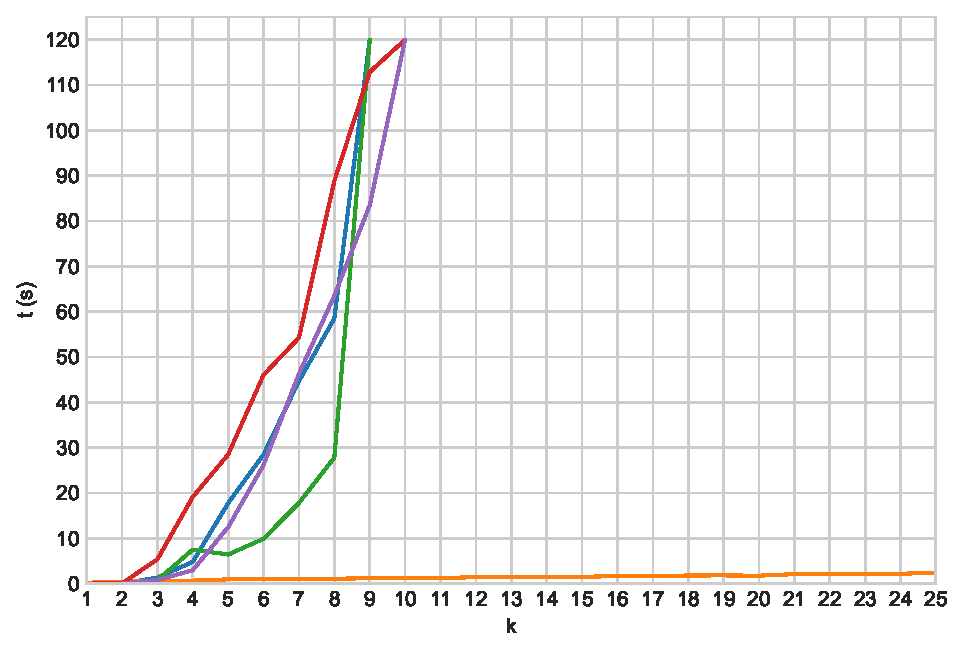
\includegraphics[width=\linewidth]{img/results/relative-comparison/75-1}
			\caption{75\% wall, one team}
			\label{fig:r-75-1}
		\end{subfigure}
		\begin{subfigure}{\graphwidth}
			\centering
			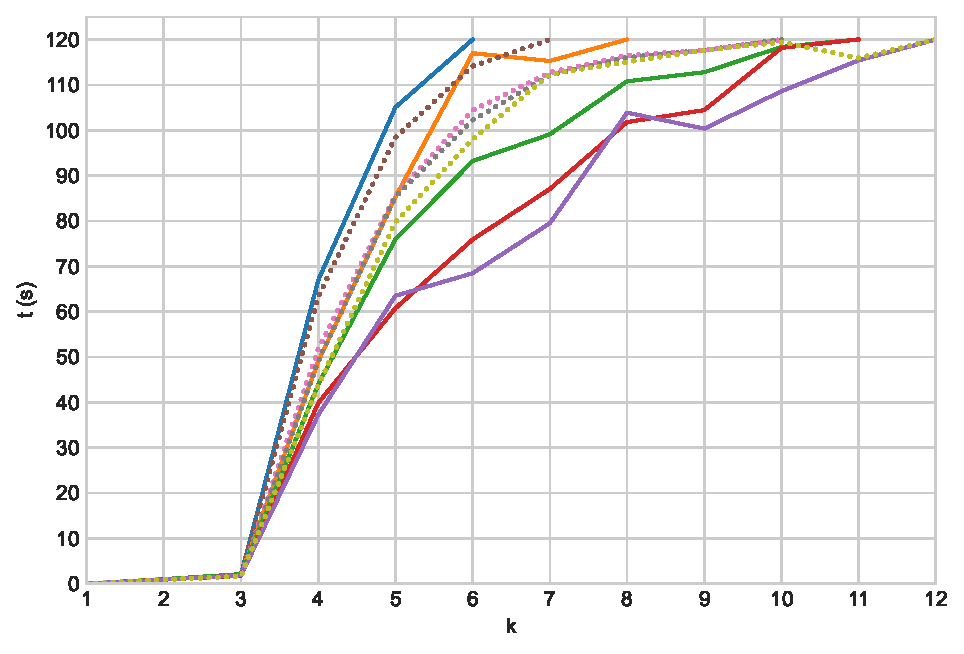
\includegraphics[width=\linewidth]{img/results/relative-comparison/75-3}
			\caption{75\% wall, three teams}
			\label{fig:r-75-3}
		\end{subfigure}
		\caption{Average solving time of MAPFM algorithms with a timeout of 120s.}
		\label{fig:r-times}
	\end{figure*}
	
	\restoregeometry
\end{document}